\section{Auswertung}
\label{sec:Auswertung}
\subsection{Frequenzspektrum von Zylindern verschiedener Länge}
Um Redundanz zu vermeiden sind statt alle zwölf nur die Frequenzspektren, wo der Zylinder die Länge $\qty{50}{\milli\meter}$ und $\qty{600}{\milli\meter}$ hat, in der Abbildung
\ref{fig:einfuehrung}
\begin{figure}
\begin{subfigure}{0.48\textwidth}%
\centering%
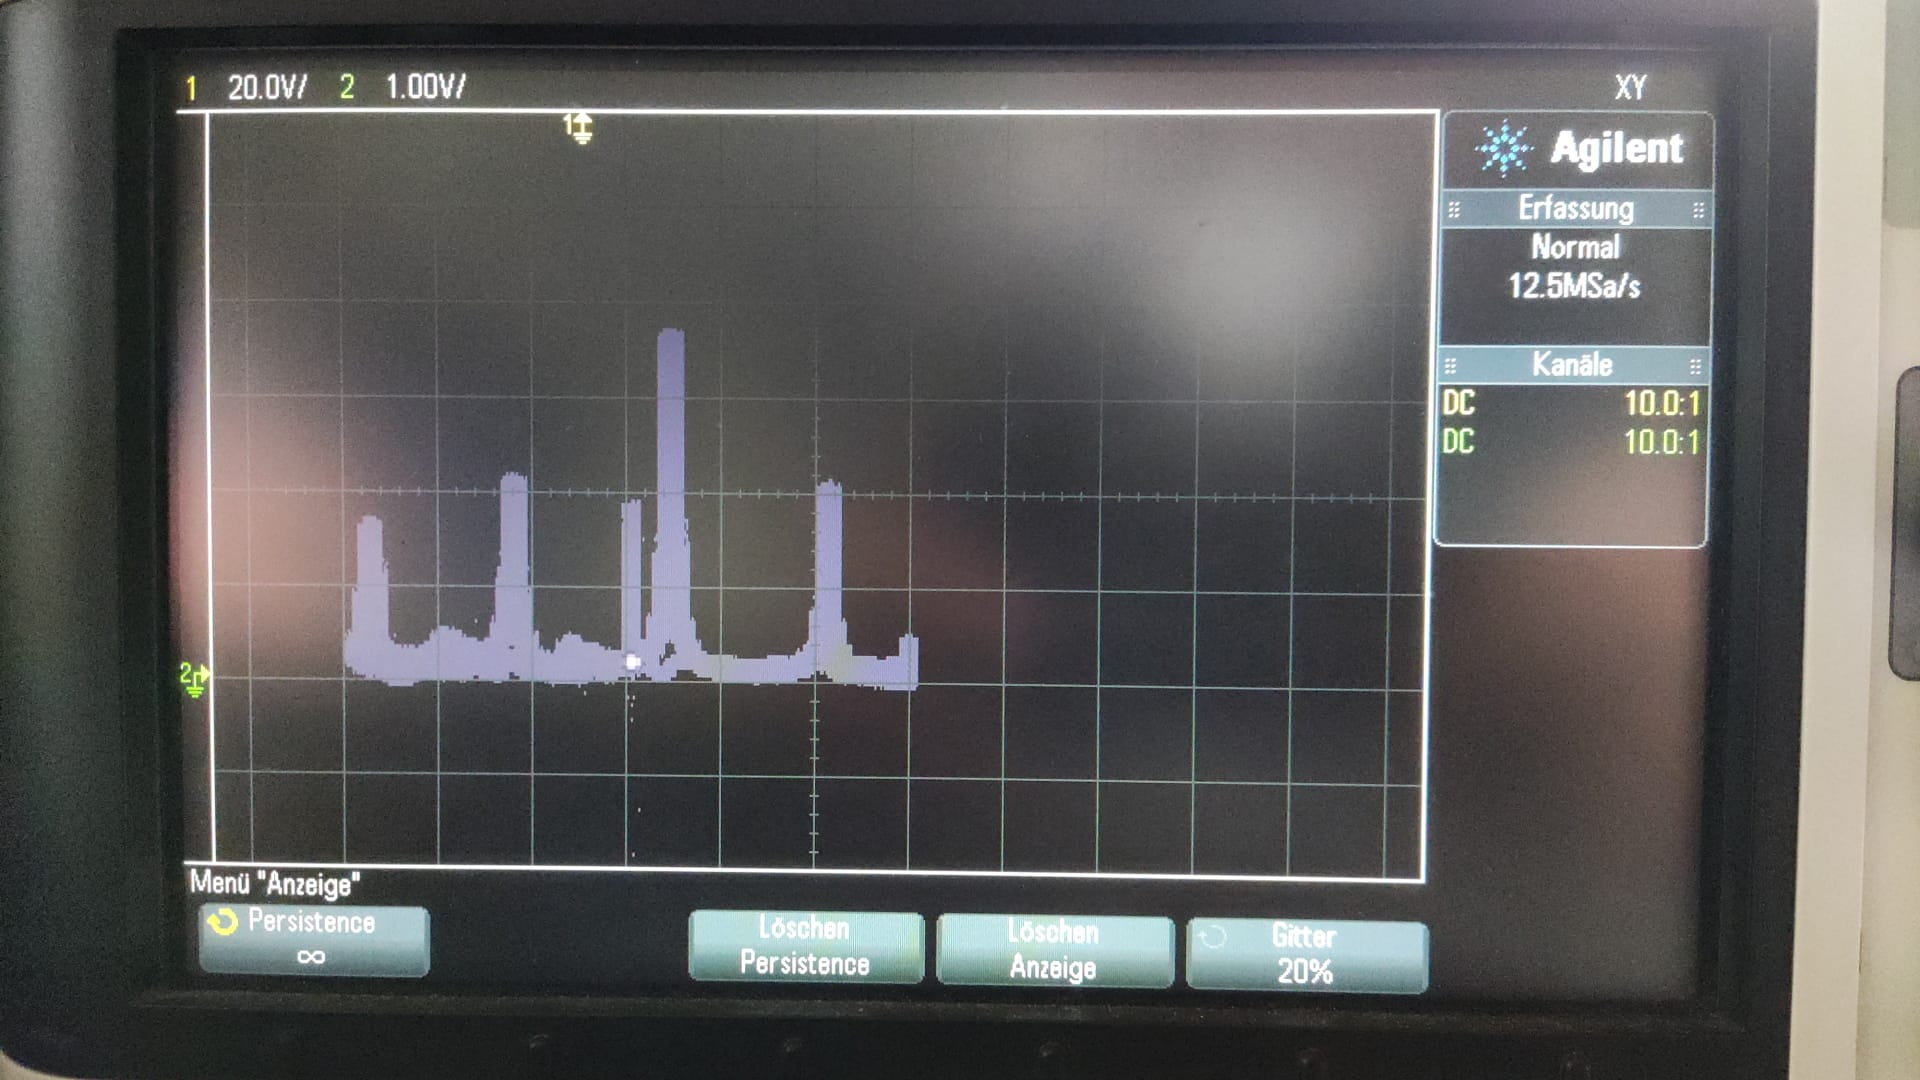
\includegraphics[height=3cm]{data_scripts/1.jpeg}%
\caption{Frequenzspektrum eines Zylinders mit der Länge $\qty{50}{\milli\meter}$}%
\label{fig:50os}%
\end{subfigure}%
\hfill% Fills available space in the center -> space between figures
\begin{subfigure}{0.48\textwidth}%
\centering%
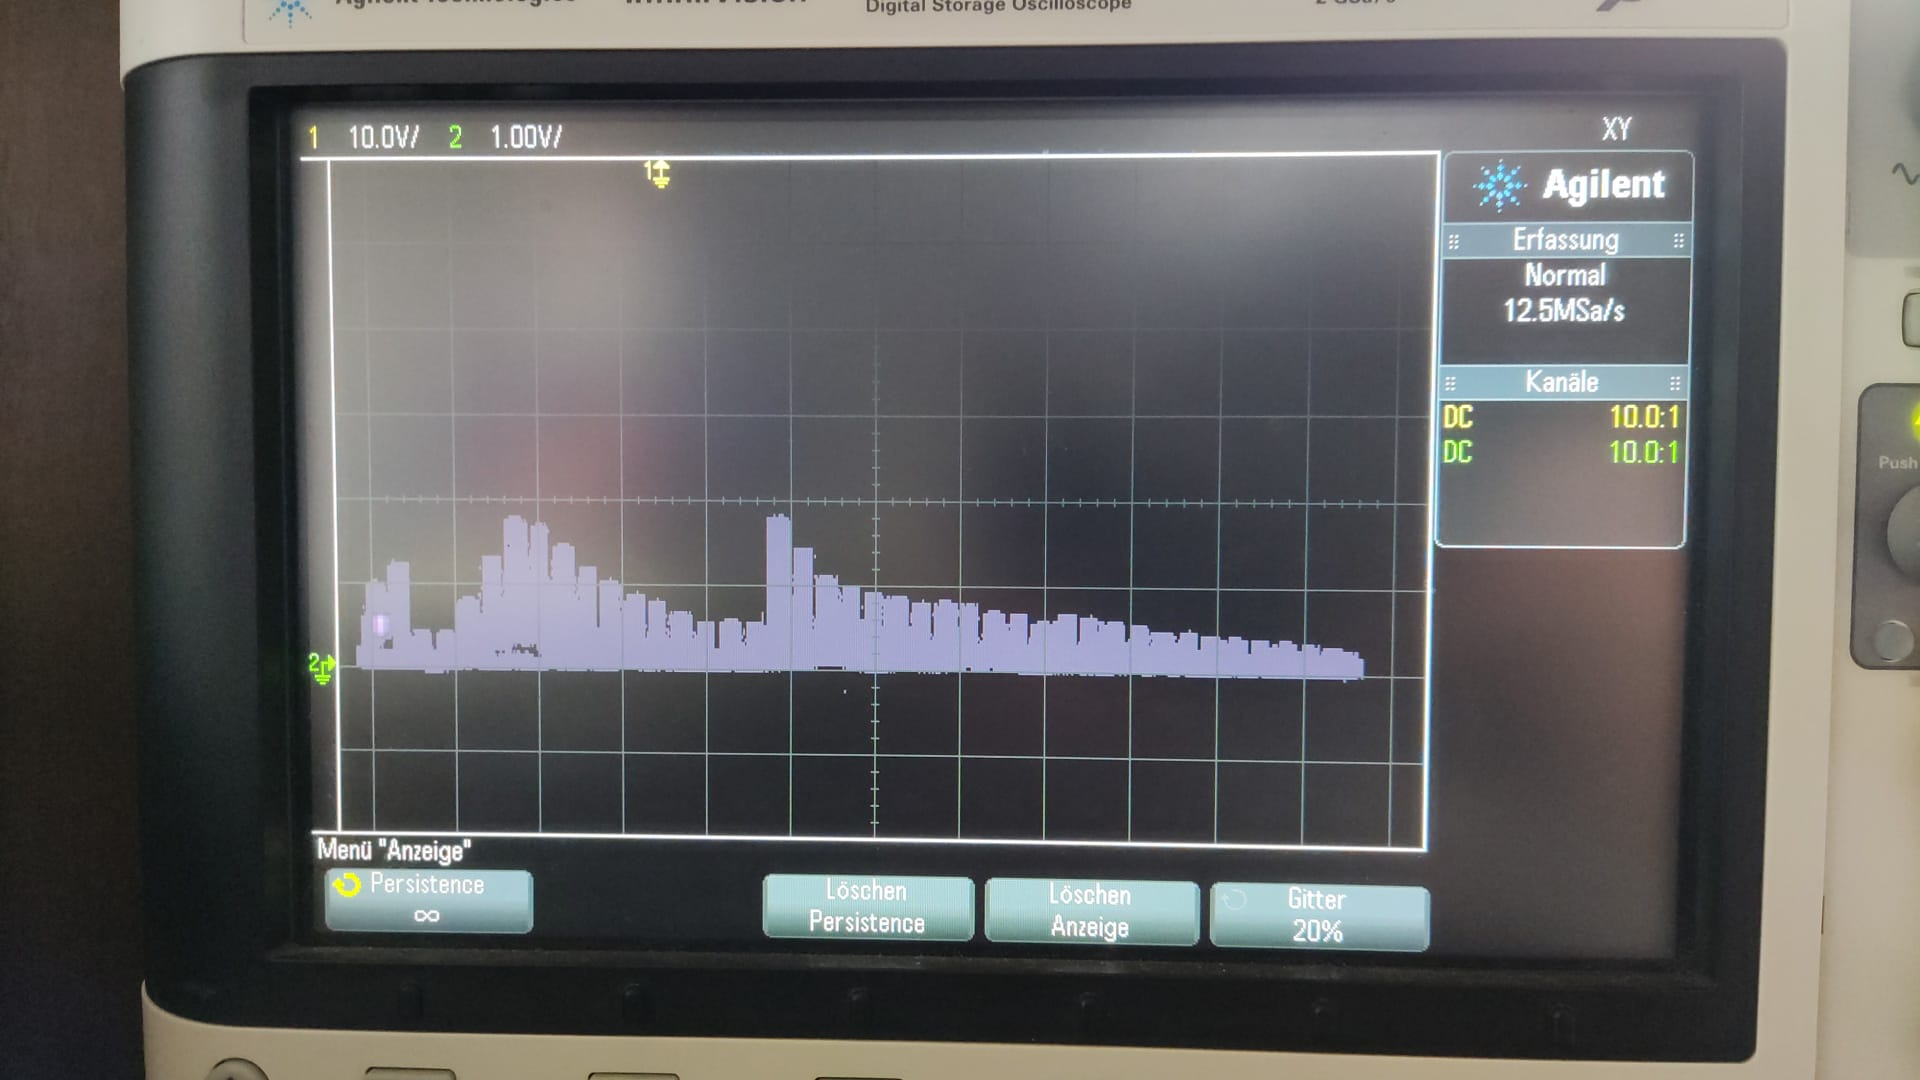
\includegraphics[height=3cm]{data_scripts/12.jpeg}%
\caption{Frequenzspektrum eines Zylinders mit der Länge $\qty{600}{\milli\meter}$}%
\label{fig:600os}%
\end{subfigure}%
\caption{Die Frequenzspektren von Zylindern mit jeweils $\qty{50}{\milli\meter}$ und $\qty{50}{\milli\meter}$, um die Frequenzspektren anderer Länge zu repräsentieren}%
\label{fig:os}%
\end{figure}%
\subsection{Winkelabhängigkeit bei dem Wasserstoffatom}
\begin{figure}
    \centering
    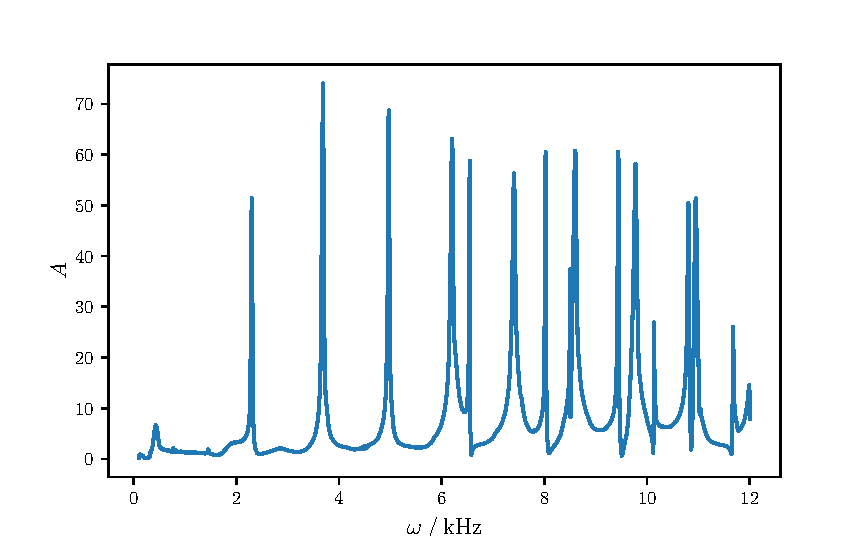
\includegraphics{build/hangle.pdf}
    \caption{Frequenzspektrum bei $\alpha = \ang{180}$}
    \label{pic:hangle}
\end{figure}
\subsection{Winkelabhängigkeit des Wasserstoffatoms}
\begin{figure}
    \centering
    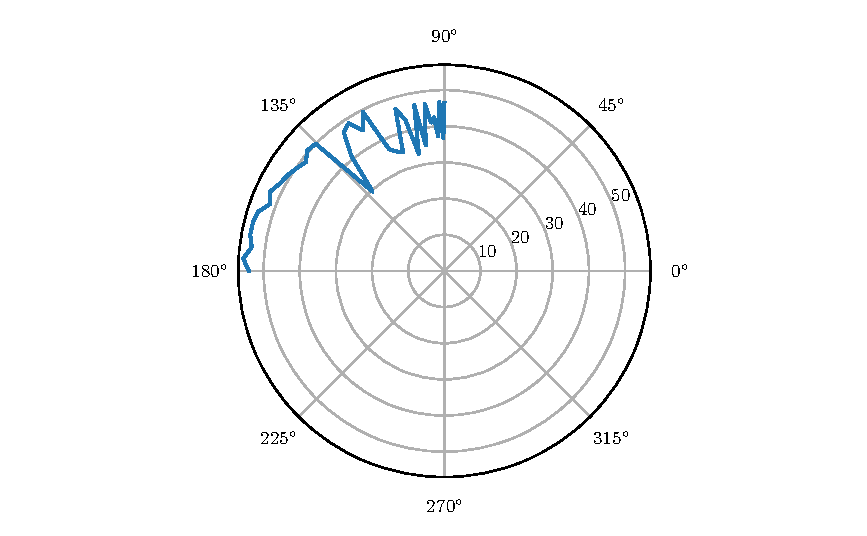
\includegraphics{build/hvarangle27.pdf}
    \caption{Polarplot des Peaks bei $\qty{2.3}{\kilo\hertz}$}
    \label{pic:hvarangle27}
\end{figure}
\begin{figure}
    \centering
    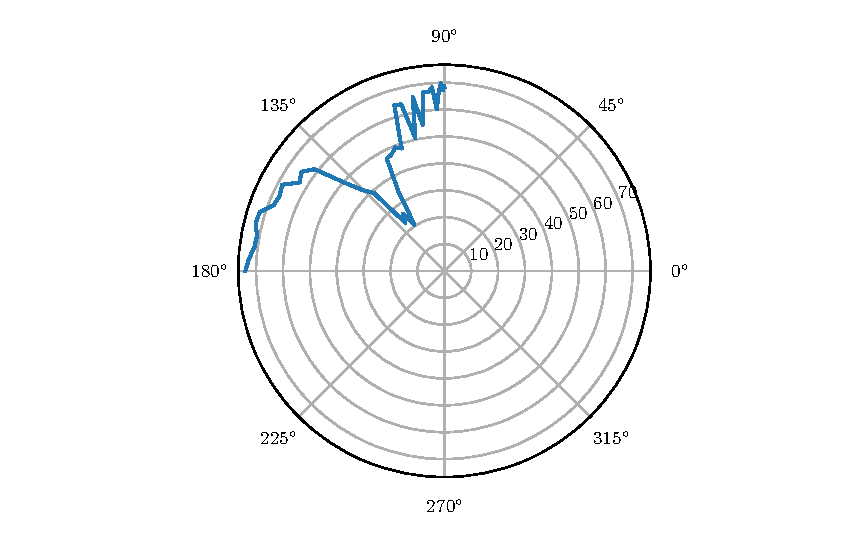
\includegraphics{build/hvarangle37.pdf}
    \caption{Polarplot des Peaks bei $\qty{3.7}{\kilo\hertz}$}
    \label{pic:hvarangle37}
\end{figure}
\begin{figure}
    \centering
    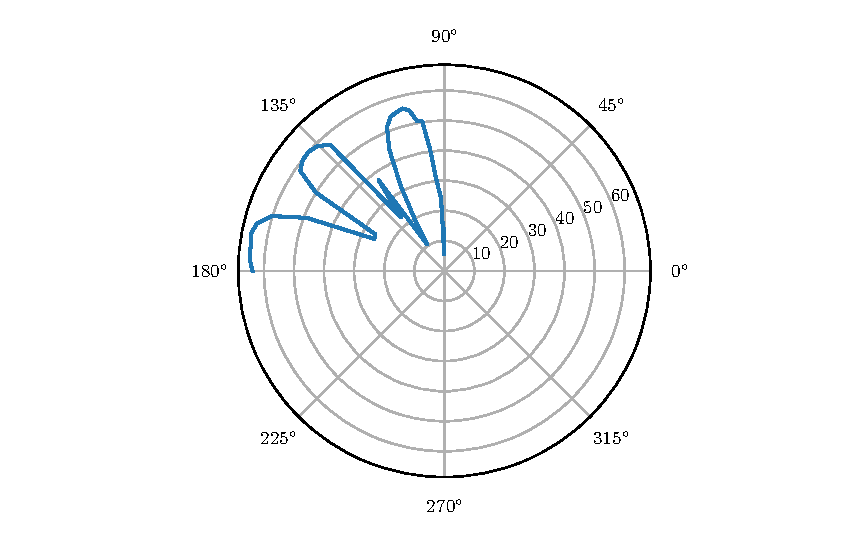
\includegraphics{build/hvarangle74.pdf}
    \caption{Polarplot des Peaks bei $\qty{7.4}{\kilo\hertz}$}
    \label{pic:hvarangle74}
\end{figure}
\begin{figure}
    \centering
    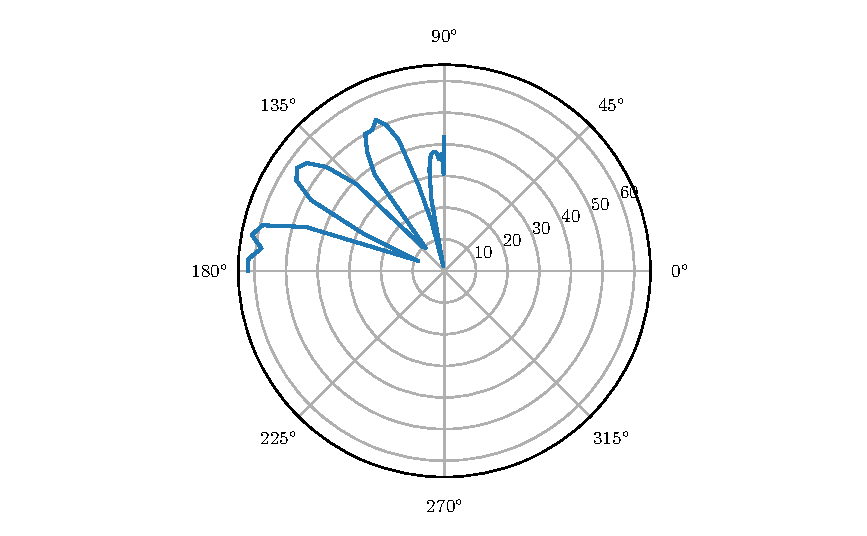
\includegraphics{build/hvarangle86.pdf}
    \caption{Polarplot des Peaks bei $\qty{8.62}{\kilo\hertz}$}
    \label{pic:hvarangle86}
\end{figure}
\subsection{Zwischenringe bei dem Wasserstoffatom}
\begin{figure}
    \centering
    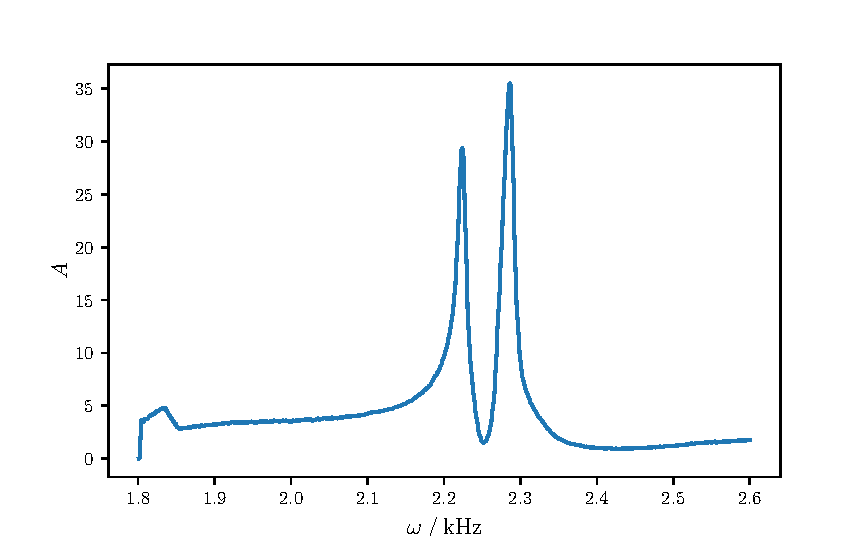
\includegraphics{build/h3ring.pdf}
    \caption{Frequenzspektrum des Wasserstoffatoms bei $\alpha = \ang{180}$ mit einem Zwischenring der Dicke $\qty{3}{\milli\meter}$}
    \label{pic:h3ring}
\end{figure}
\begin{figure}
    \centering
    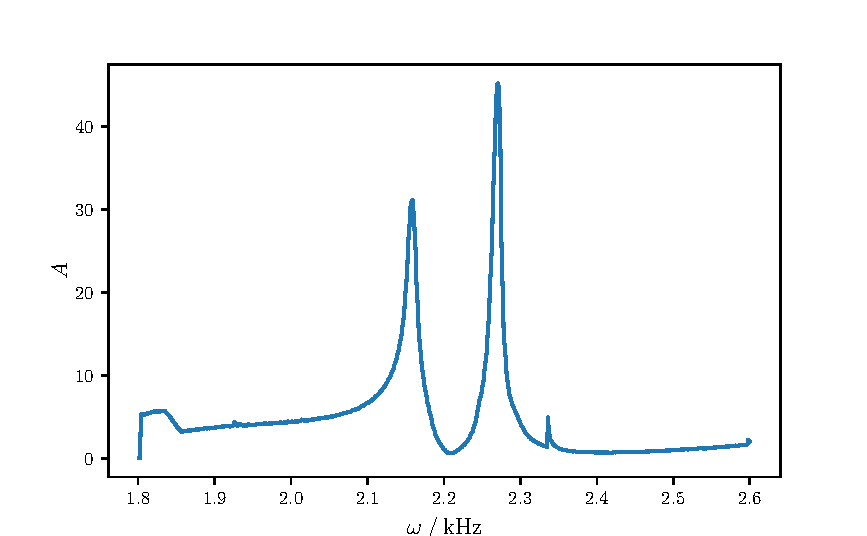
\includegraphics{build/h6ring.pdf}
    \caption{Frequenzspektrum des Wasserstoffatoms bei $\alpha = \ang{180}$ mit einem Zwischenring der Dicke $\qty{6}{\milli\meter}$}
    \label{pic:h6ring}
\end{figure}
\begin{figure}
    \centering
    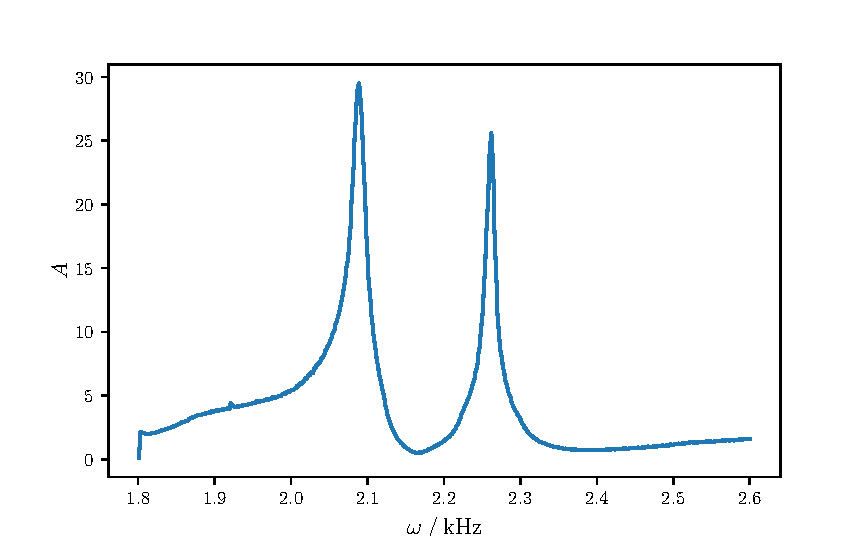
\includegraphics{build/h9ring.pdf}
    \caption{Frequenzspektrum des Wasserstoffatoms bei $\alpha = \ang{180}$ mit einem Zwischenring der Dicke $\qty{9}{\milli\meter}$}
    \label{pic:h9ring}
\end{figure}
\begin{figure}
    \centering
    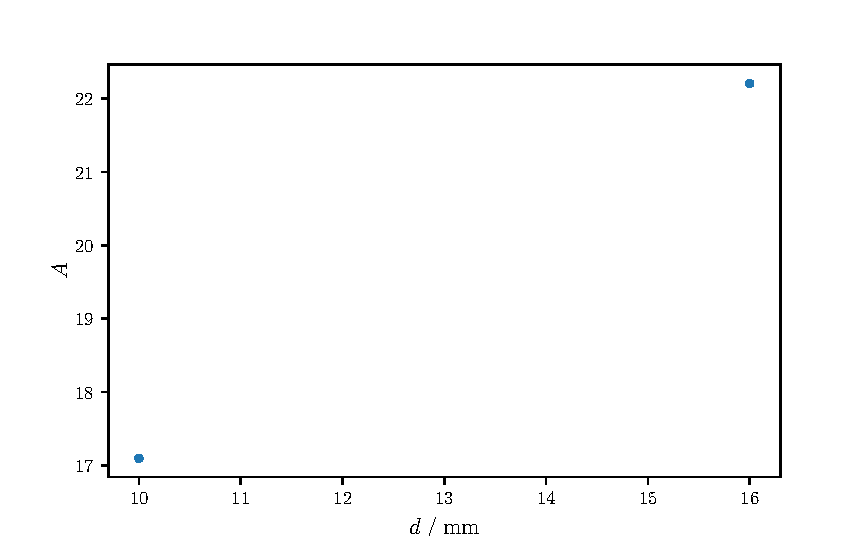
\includegraphics{build/h2dia.pdf}
    \caption{Resonanzamplitude des Wasserstoffmoleküls bei $\alpha = \ang{180}$ in Abhängigkeit des Blendendurchmessers}
    \label{pic:h9ring}
\end{figure}
\begin{figure}
    \centering
    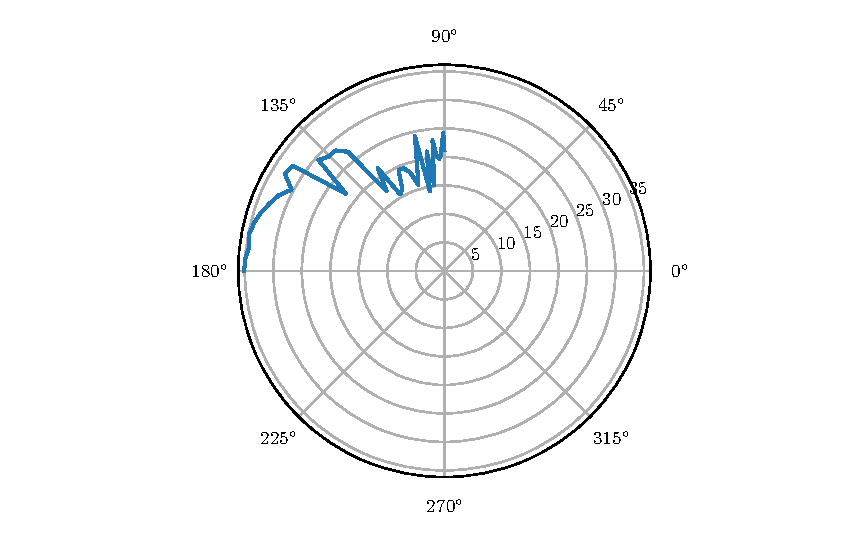
\includegraphics{build/h2varangle.pdf}
    \caption{Polarplot des Peaks bei $\qty{2.3}{\kilo\hertz}$}
    \label{pic:h9ring}
\end{figure}
\begin{figure}
    \begin{subfigure}{0.48\textwidth}%
    \centering%
    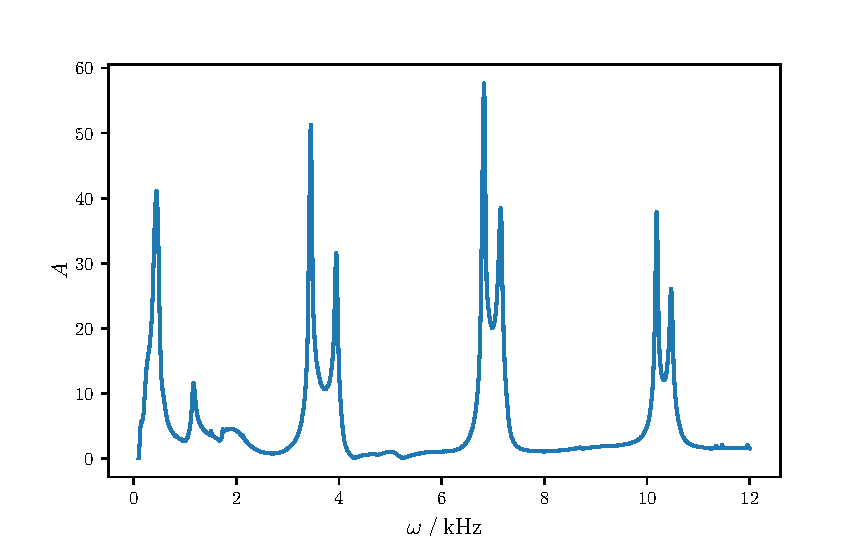
\includegraphics[height=5cm]{build/2c1b10.pdf}%
    \caption{Frequenzspektren eines 1-dimensionalen Fesktörpers bestehend aus zwei $\qty{50}{\milli\meter}$ Zylinder und einer $\qty{10}{\milli\meter}$ Blende.}%
    \label{fig:2c1b10}%
    \end{subfigure}%
    \hfill% Fills available space in the center -> space between figures
    \begin{subfigure}{0.48\textwidth}%
    \centering%
    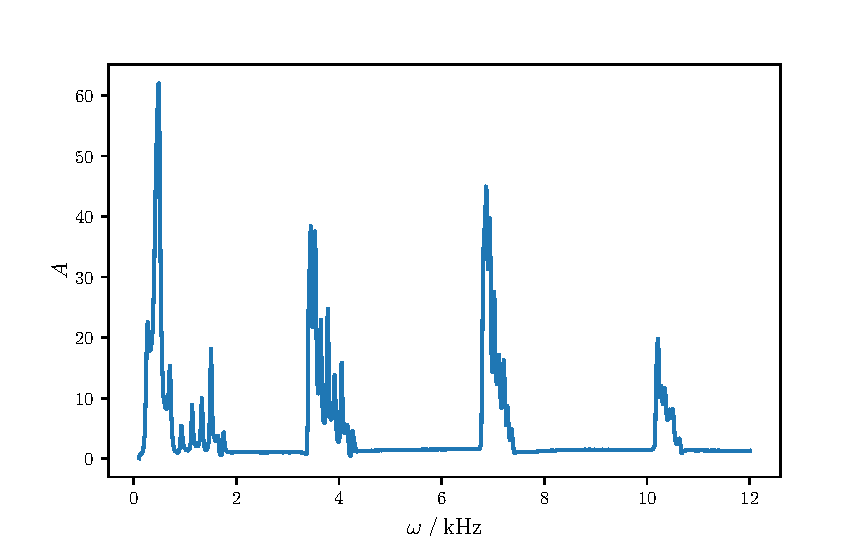
\includegraphics[height=5cm]{build/10c9b10.pdf}%
    \caption{Frequenzspektrum eines 1-dimensionalen Fesktörpers bestehend aus zehn $\qty{50}{\milli\meter}$ Zylinder und neun $\qty{10}{\milli\meter}$ Blende.}%
    \label{fig:2c1b}%
    \end{subfigure}%
    \caption{Die Frequenzspektrum Festkörpern bestehen aus zwei bzw. zehn $\qty{50}{\milli\meter}$ Zylinder mit einer bzw. neun $\qty{13}{\milli\meter}$ Blenden, um die 
    Frequenzspektren Festkörper, welche eine Länge zwischen diesen beiden Extremen haben, zu repräsentieren.}%
    \label{fig:10mm}
\end{figure}%
\begin{figure}
    \begin{subfigure}{0.48\textwidth}%
    \centering%
    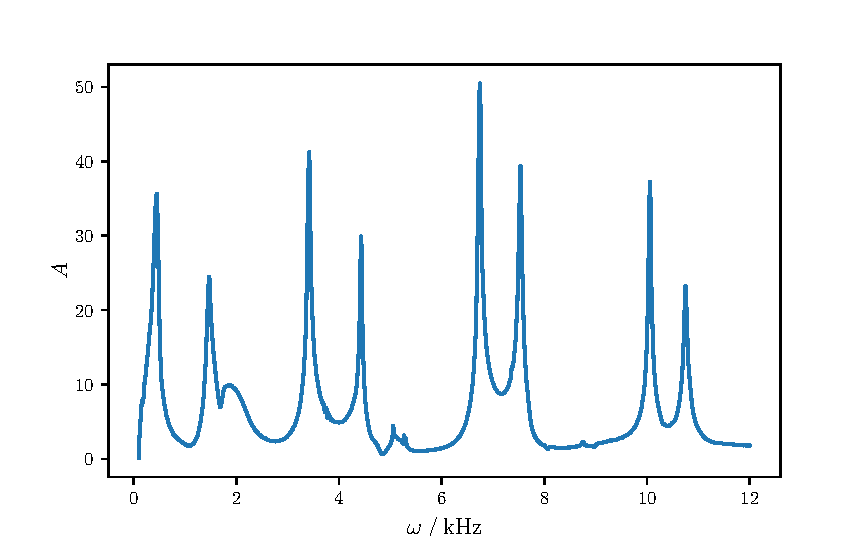
\includegraphics[height=5cm]{build/2c1b.pdf}%
    \caption{Frequenzspektren eines 1-dimensionalen Fesktörpers bestehend aus zwei $\qty{50}{\milli\meter}$ Zylinder und einer $\qty{16}{\milli\meter}$ Blende.}%
    \label{fig:2c1b}%
    \end{subfigure}%
    \hfill% Fills available space in the center -> space between figures
    \begin{subfigure}{0.48\textwidth}%
    \centering%
    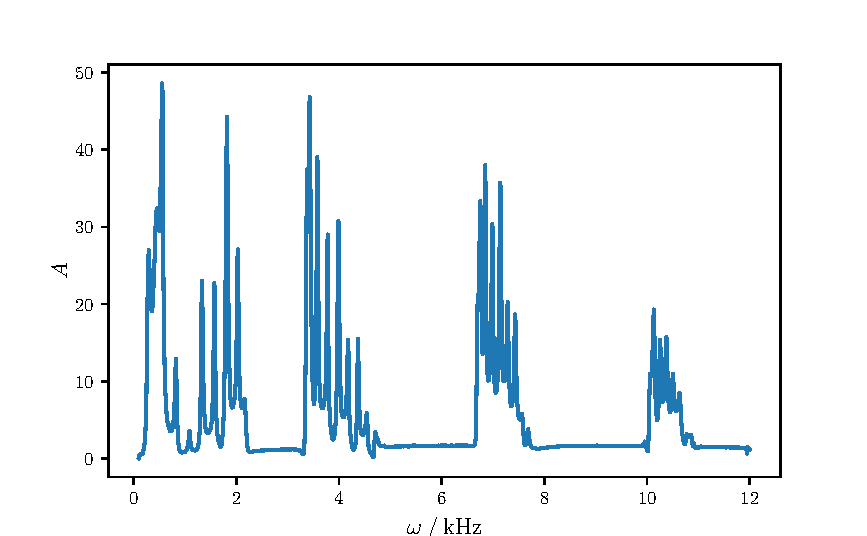
\includegraphics[height=5cm]{build/10c9b.pdf}%
    \caption{Frequenzspektrum eines 1-dimensionalen Fesktörpers bestehend aus zehn $\qty{50}{\milli\meter}$ Zylinder und neun $\qty{13}{\milli\meter}$ Blende.}%
    \label{fig:2c1b}%
    \end{subfigure}%
    \caption{Die Frequenzspektrum Festkörpern bestehen aus zwei bzw. zehn $\qty{50}{\milli\meter}$ Zylinder mit einer bzw. neun $\qty{13}{\milli\meter}$ Blenden, um die 
    Frequenzspektren Festkörper, welche eine Länge zwischen diesen beiden Extremen haben, zu repräsentieren.}%
    \label{fig:13mm}
\end{figure}%
\begin{figure}
    \begin{subfigure}{0.48\textwidth}%
    \centering%
    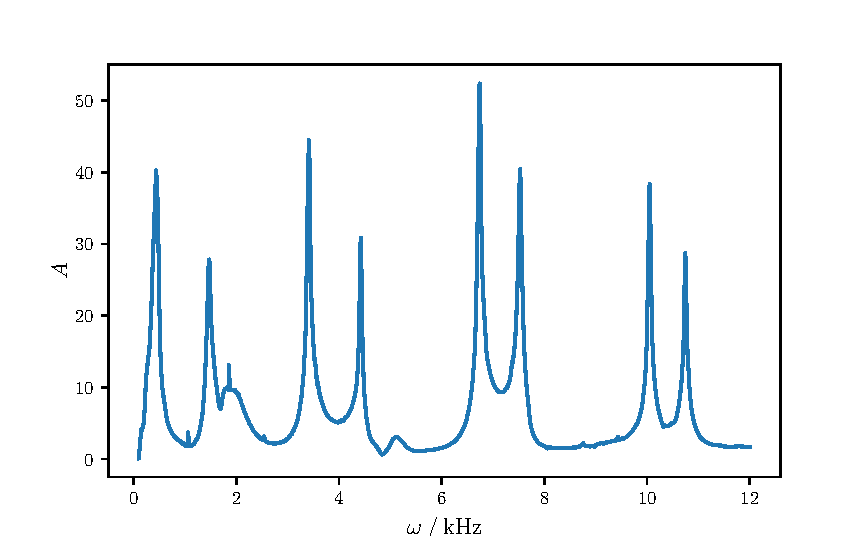
\includegraphics[height=5cm]{build/2c1b16.pdf}%
    \caption{Frequenzspektren eines 1-dimensionalen Fesktörpers bestehend aus zwei $\qty{50}{\milli\meter}$ Zylinder und einer $\qty{16}{\milli\meter}$ Blende.}%
    \label{fig:2c1b16}%
    \end{subfigure}%
    \hfill% Fills available space in the center -> space between figures
    \begin{subfigure}{0.48\textwidth}%
    \centering%
    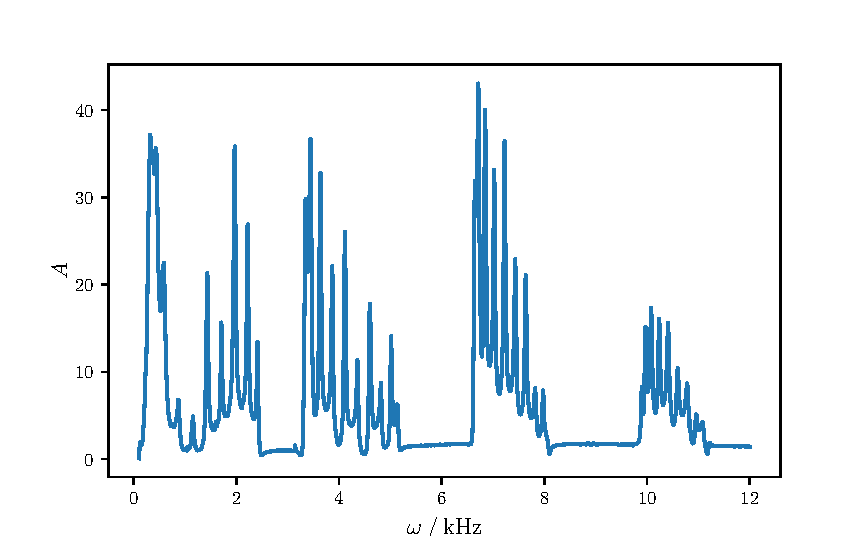
\includegraphics[height=5cm]{build/10c9b16.pdf}%
    \caption{Frequenzspektrum eines 1-dimensionalen Fesktörpers bestehend aus zehn $\qty{50}{\milli\meter}$ Zylinder und neun $\qty{16}{\milli\meter}$ Blende.}%
    \label{fig:2c1b16}%
    \end{subfigure}%
    \caption{Die Frequenzspektrum Festkörpern bestehen aus zwei bzw. zehn $\qty{50}{\milli\meter}$ Zylinder mit einer bzw. neun $\qty{16}{\milli\meter}$ Blenden, um die 
    Frequenzspektren Festkörper, welche eine Länge zwischen diesen beiden Extremen haben, zu repräsentieren.}%
    \label{fig:16mm}
\end{figure}%
\begin{figure}
    \begin{subfigure}{0.48\textwidth}%
        \centering%
        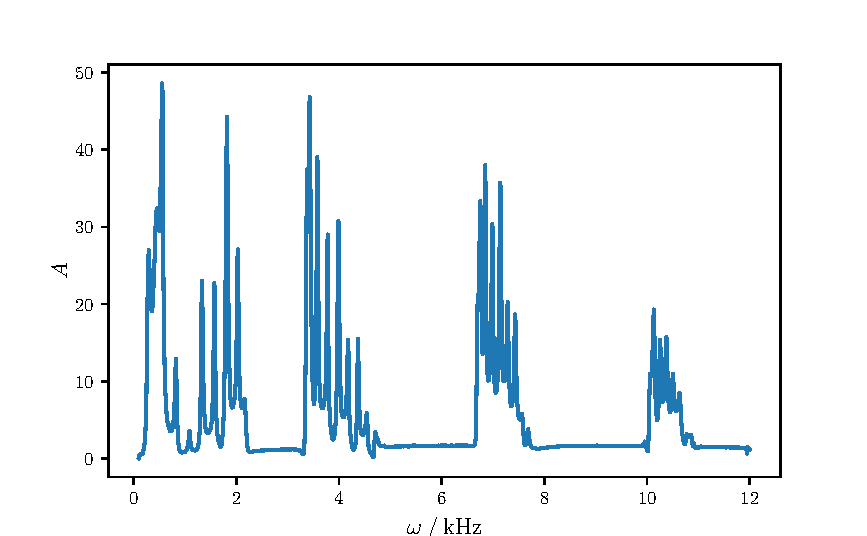
\includegraphics[height=5cm]{build/10c9b.pdf}%
        \caption{Frequenzspektren eines 1-dimensionalen Fesktörpers bestehend aus zwei $\qty{50}{\milli\meter}$ Zylinder und einer $\qty{16}{\milli\meter}$ Blende.}%
        \label{fig:10c9b}%
    \end{subfigure}%
    \hfill% Fills available space in the center -> space between figures
    \begin{subfigure}{0.48\textwidth}%
        \centering%
        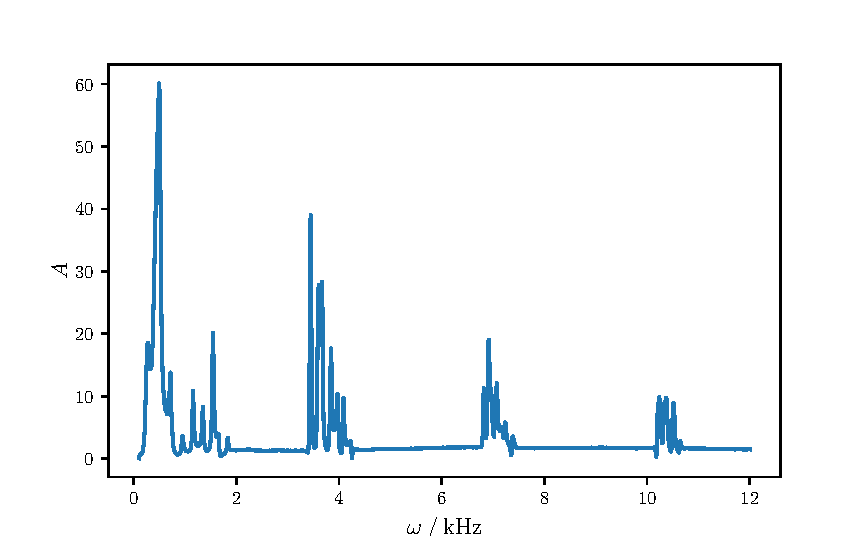
\includegraphics[height=5cm]{build/10c9b375.pdf}
        \caption{Frequenzspektrum eines 1-dimensionalen Fesktörpers bestehend aus zehn $\qty{50}{\milli\meter}$ Zylinder und neun $\qty{16}{\milli\meter}$ Blende.}%
        \label{fig:10c9b375}
    \end{subfigure} \\
    \begin{subfigure}{0.48\textwidth}%
        \centering%
        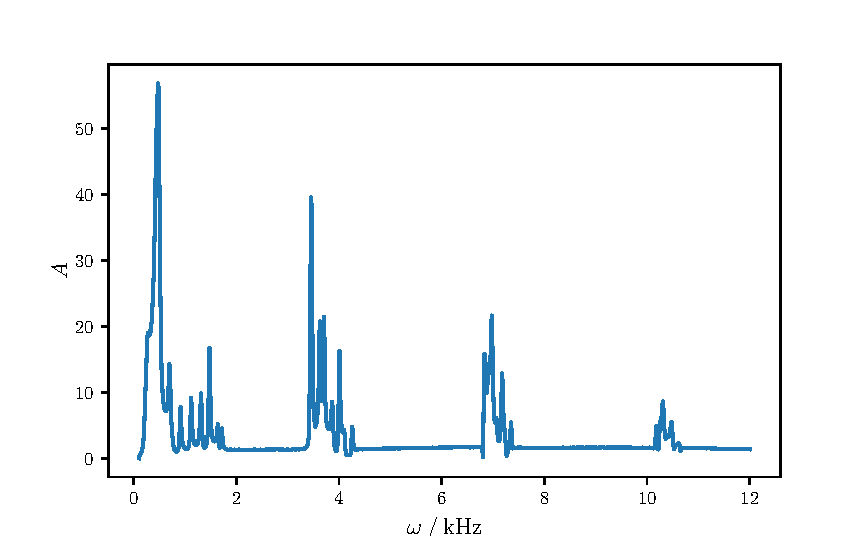
\includegraphics[height=5cm]{build/10c9b625.pdf}%
        \caption{Frequenzspektren eines 1-dimensionalen Fesktörpers bestehend aus zwei $\qty{50}{\milli\meter}$ Zylinder und einer $\qty{16}{\milli\meter}$ Blende.}%
        \label{fig:10c9b625}
    \end{subfigure}%
    \hfill
    \begin{subfigure}{0.48\textwidth}%
        \centering%
        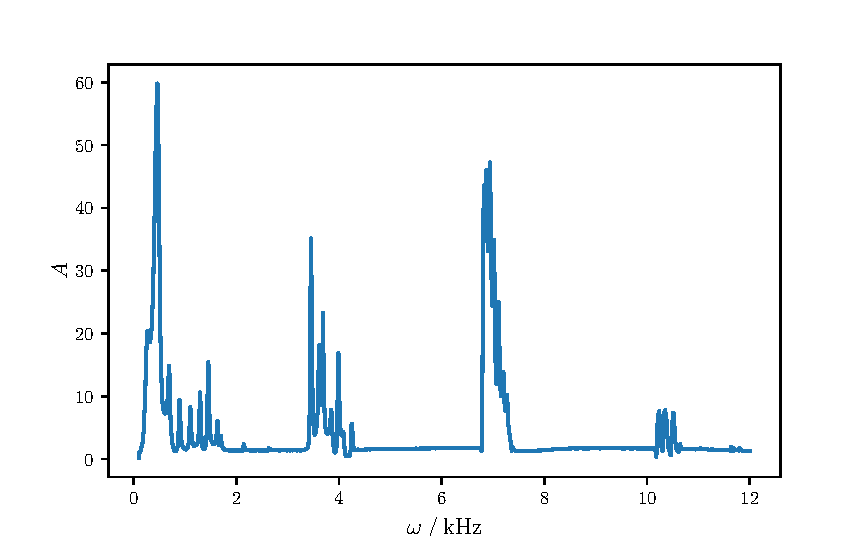
\includegraphics[height=5cm]{build/10c9b75.pdf}%
        \caption{Frequenzspektren eines 1-dimensionalen Fesktörpers bestehend aus zwei $\qty{50}{\milli\meter}$ Zylinder und einer $\qty{16}{\milli\meter}$ Blende.}%
        \label{fig:10c9b75}
    \end{subfigure}%
    \caption{Die Frequenzspektrum der Festkörpern bestehen aus zwei bzw. zehn $\qty{50}{\milli\meter}$ Zylinder mit einer bzw. neun $\qty{16}{\milli\meter}$ Blenden, um die 
            Frequenzspektren Festkörper, welche eine Länge zwischen diesen beiden Extremen haben, zu repräsentieren.}%
    \label{fig:austauschen}
\end{figure}%
\begin{figure}
    \centering
    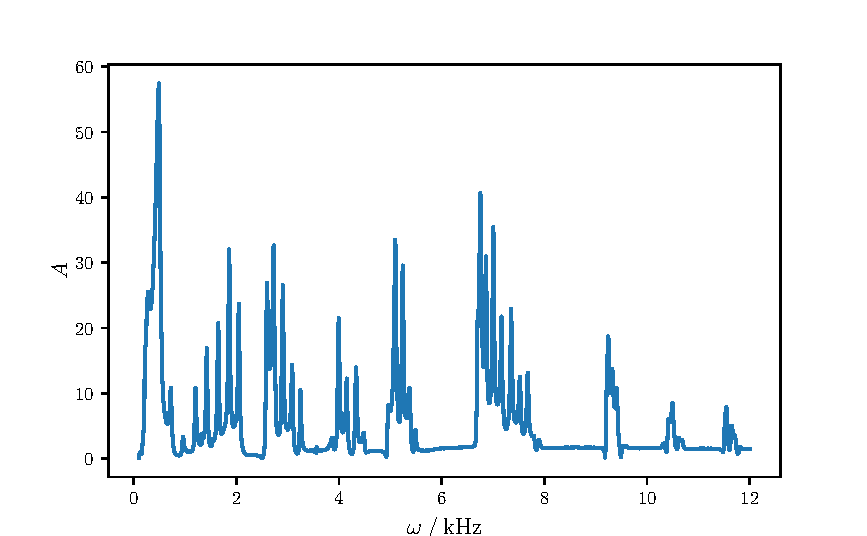
\includegraphics{build/5075.pdf}
    \caption{Abwechselnd 5075$\qty{2.3}{\kilo\hertz}$}
    \label{pic:5075}
\end{figure}
\begin{figure}
    \begin{subfigure}{0.48\textwidth}%
        \centering%
        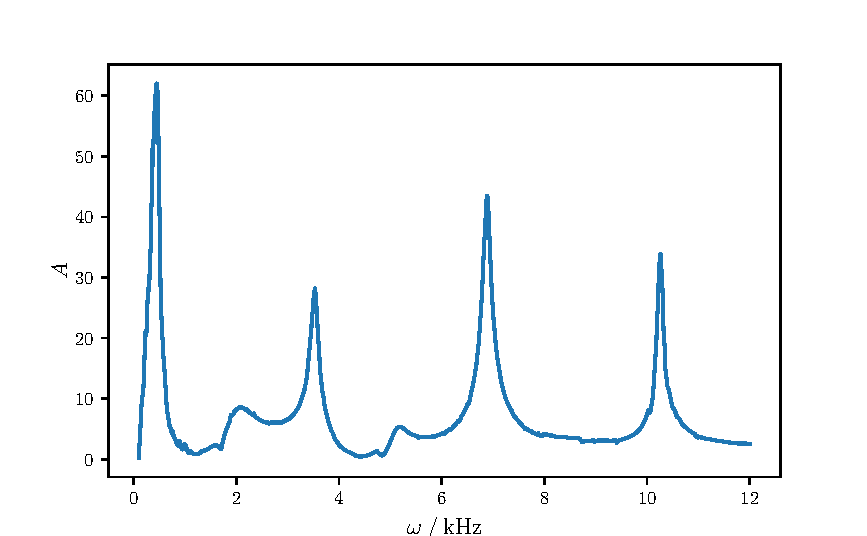
\includegraphics[height=5cm]{build/50single.pdf}%
        \caption{Frequenzspektren eines 1-dimensionalen Fesktörpers bestehend aus zwei $\qty{50}{\milli\meter}$ Zylinder und einer $\qty{16}{\milli\meter}$ Blende.}%
        \label{fig:50sinlge}%
    \end{subfigure}%
    \hfill% Fills available space in the center -> space between figures
    \begin{subfigure}{0.48\textwidth}%
        \centering%
        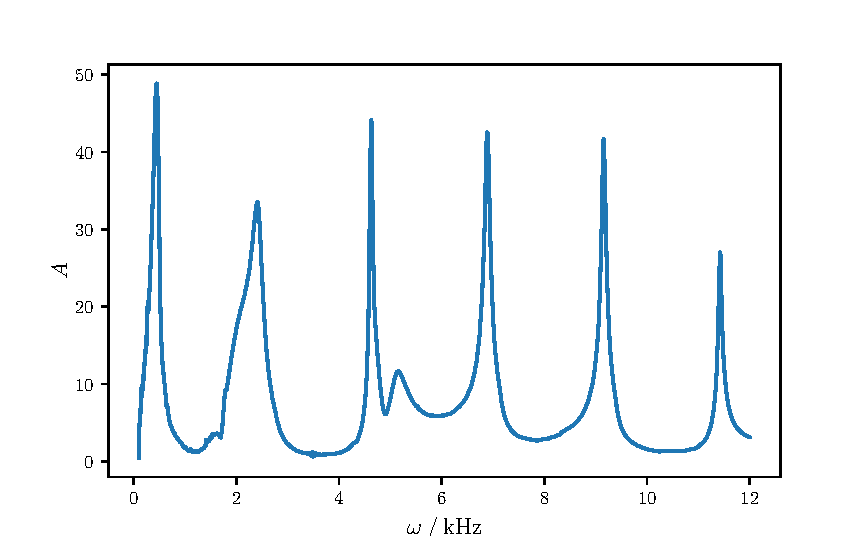
\includegraphics[height=5cm]{build/75single.pdf}%
        \caption{Frequenzspektrum eines einzelnen $\qty{50}{\milli\meter}$ Zylinders}%
        \label{fig:75single}%
    \end{subfigure}%
    \caption{Die Frequenzspektrum von einzelnen $\qty{50}{\milli\meter}$ bzw. $\qty{75}{\milli\meter}$ Zylindern.}%
    \label{fig:75and50single}
\end{figure}%